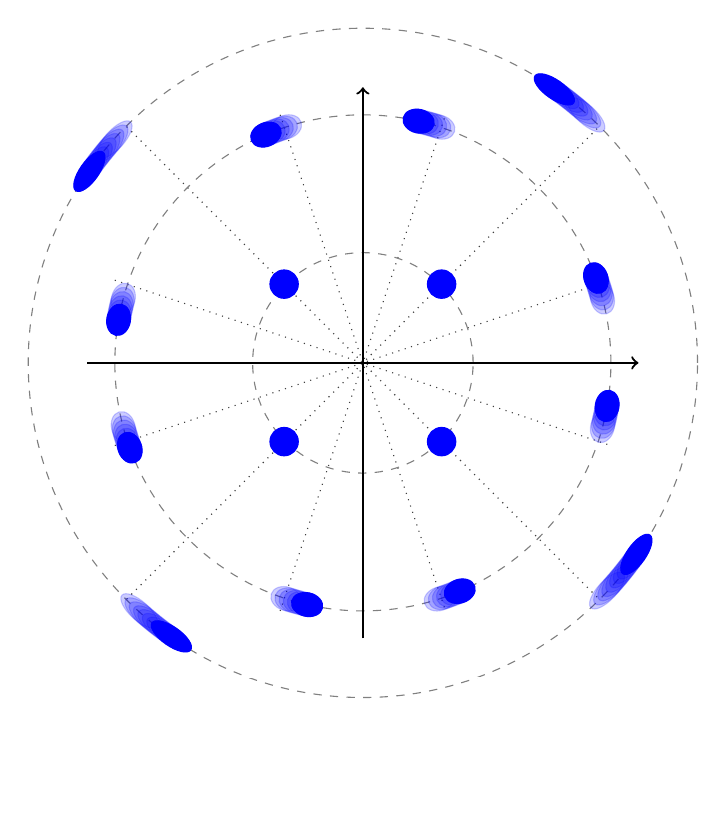
\begin{tikzpicture}%[scale = 0.5]
    \draw[gray!50!black, dotted] (-3,-3) --++ (6,6);
    \draw[gray!50!black, dotted] (-3,3) --++ (6,-6);
    \draw[gray!50!black, dotted] (-1.05,-3.15) --++ (2.1,6.3);
    \draw[gray!50!black, dotted] (-1.05,3.15) --++ (2.1,-6.3);
    \draw[gray!50!black, dotted] (-3.15,-1.05) --++ (6.3,2.1);
    \draw[gray!50!black, dotted] (-3.15,1.05) --++ (6.3,-2.1);
    
    \draw[gray, dashed] (0,0) circle (1.4);
    \draw[gray, dashed] (0,0) circle (3.15);
    \draw[gray, dashed] (0,0) circle (4.25);

%%%%%%%%%%%%%%%%%%%%%%%%%% INNER POINTS
    \draw[fill = blue, color = blue] (-1,-1) circle (0.18);
    \draw[fill = blue, color = blue] (-1,1) circle (0.18);
    \draw[fill = blue, color = blue] (1,1) circle (0.18);
    \draw[fill = blue, color = blue] (1,-1) circle (0.18);

%%%%%%%%%%%%%%%%%%%%%%%%%% INTERMEDIATE POINTS

    \draw[fill = blue, color = blue, rotate around={20:({3.15*cos(20)}, {3.15*sin(20)})}]
      ({3.15*cos(20)}, {3.15*sin(20)}) ellipse (0.15 and 0.2);
    \draw[fill = blue, color = blue, rotate around={-10:({3.15*cos(10)}, {-3.15*sin(10)})}]
      ({3.15*cos(10)}, {-3.15*sin(10)}) ellipse (0.15 and 0.2);
    \draw[fill = blue, color = blue, rotate around={170:({3.15*cos(170)}, {3.15*sin(170)})}]
      ({3.15*cos(170)}, {3.15*sin(170)}) ellipse (0.15 and 0.2);
    \draw[fill = blue, color = blue, rotate around={-160:({3.15*cos(160)}, {-3.15*sin(160)})}]
      ({3.15*cos(160)}, {-3.15*sin(160)}) ellipse (0.15 and 0.2);

    \foreach \a in {15,...,20} {
      \draw[fill = blue,color = blue, opacity=0.2,
        rotate around={\a + 90:( {3.15*cos(\a)}, {3.15*sin(\a)} )}
      ]
      ({3.15*cos(\a)}, {3.15*sin(\a)}) ellipse (0.2 and 0.15);
    }

    \foreach \a in {-15,...,-10} {
      \draw[fill = blue,color = blue, opacity=0.2,
        rotate around={\a + 90:( {3.15*cos(\a)}, {3.15*sin(\a)} )}
      ]
      ({3.15*cos(\a)}, {3.15*sin(\a)}) ellipse (0.2 and 0.15);
    }

    \foreach \a in {165,...,170} {
      \draw[fill = blue,color = blue, opacity=0.2,
        rotate around={\a + 90:( {3.15*cos(\a)}, {3.15*sin(\a)} )}
      ]
      ({3.15*cos(\a)}, {3.15*sin(\a)}) ellipse (0.2 and 0.15);
    }

    \foreach \a in {-165,...,-160} {
      \draw[fill = blue,color = blue, opacity=0.2,
        rotate around={\a + 90:( {3.15*cos(\a)}, {3.15*sin(\a)} )}
      ]
      ({3.15*cos(\a)}, {3.15*sin(\a)}) ellipse (0.2 and 0.15);
    }
    
    \draw[fill = blue, color = blue, rotate around={77:({3.15*cos(77)}, {3.15*sin(77)})}]
      ({3.15*cos(77)}, {3.15*sin(77)}) ellipse (0.15 and 0.2);
    \draw[fill = blue, color = blue, rotate around={-72:({3.15*cos(67)}, {-3.15*sin(67)})}]
      ({3.15*cos(67)}, {-3.15*sin(67)}) ellipse (0.15 and 0.2);
    \draw[fill = blue, color = blue, rotate around={113:({3.15*cos(113)}, {3.15*sin(113)})}]
      ({3.15*cos(113)}, {3.15*sin(113)}) ellipse (0.15 and 0.2);
    \draw[fill = blue, color = blue, rotate around={-103:({3.15*cos(103)}, {-3.15*sin(103)})}]
      ({3.15*cos(103)}, {-3.15*sin(103)}) ellipse (0.15 and 0.2);


    \foreach \a in {72,...,77} {
      \draw[fill = blue,color = blue, opacity=0.2,
        rotate around={\a + 90:( {3.15*cos(\a)}, {3.15*sin(\a)} )}
      ]
      ({3.15*cos(\a)}, {3.15*sin(\a)}) ellipse (0.2 and 0.15);
    }
    
    \foreach \a in {108,...,113} {
      \draw[fill = blue,color = blue, opacity=0.2,
        rotate around={\a + 90:( {3.15*cos(\a)}, {3.15*sin(\a)} )}
      ]
      ({3.15*cos(\a)}, {3.15*sin(\a)}) ellipse (0.2 and 0.15);
    }
    
    \foreach \a in {-72,...,-67} {
      \draw[fill = blue,color = blue, opacity=0.2,
        rotate around={\a + 90:( {3.15*cos(\a)}, {3.15*sin(\a)} )}
      ]
      ({3.15*cos(\a)}, {3.15*sin(\a)}) ellipse (0.2 and 0.15);
    }
    
    \foreach \a in {-108,...,-103} {
      \draw[fill = blue,color = blue, opacity=0.2,
        rotate around={\a + 90:( {3.15*cos(\a)}, {3.15*sin(\a)} )}
      ]
      ({3.15*cos(\a)}, {3.15*sin(\a)}) ellipse (0.2 and 0.15);
    }


%%%%%%%%%%%%%%%%%%%%%%%%%% OUTER POINTS
    \draw[fill = blue, color = blue, rotate around={55:({4.24*cos(55)}, {4.24*sin(55)})}]
      ({4.24*cos(55)}, {4.24*sin(55)}) ellipse (0.12 and 0.3);
    \draw[fill = blue, color = blue, rotate around={-35:({4.24*cos(35)}, {-4.24*sin(35)})}]
      ({4.24*cos(35)}, {-4.24*sin(35)}) ellipse (0.12 and 0.3);
    \draw[fill = blue, color = blue, rotate around={145:({4.24*cos(145)}, {4.24*sin(145)})}]
      ({4.24*cos(145)}, {4.24*sin(145)}) ellipse (0.12 and 0.3);
    \draw[fill = blue, color = blue, rotate around={-125:({4.24*cos(125)}, {-4.24*sin(125)})}]
      ({4.24*cos(125)}, {-4.24*sin(125)}) ellipse (0.12 and 0.3);


    \foreach \a in {48,...,55} {
      \draw[fill = blue,color = blue, opacity=0.2, rotate around={\a + 90:( {4.24*cos(\a)}, {4.24*sin(\a)} )}
      ]
      ({4.24*cos(\a)}, {4.24*sin(\a)}) ellipse (0.3 and 0.12);
    }
    
    \foreach \a in {138,...,145} {
      \draw[fill = blue,color = blue, opacity=0.2, rotate around={\a + 90:( {4.24*cos(\a)}, {4.24*sin(\a)} )}
      ]
      ({4.24*cos(\a)}, {4.24*sin(\a)}) ellipse (0.3 and 0.12);
    }
    
    
    \foreach \a in {-43,...,-35} {
      \draw[fill = blue,color = blue, opacity=0.2, rotate around={\a + 90:( {4.24*cos(\a)}, {4.24*sin(\a)} )}
      ]
      ({4.24*cos(\a)}, {4.24*sin(\a)}) ellipse (0.3 and 0.12);
    }
    
    
    \foreach \a in {-132,...,-125} {
      \draw[fill = blue,color = blue, opacity=0.2, rotate around={\a + 90:( {4.24*cos(\a)}, {4.24*sin(\a)} )}
      ]
      ({4.24*cos(\a)}, {4.24*sin(\a)}) ellipse (0.3 and 0.12);
    }





    \draw[->, thick] (-3.5,0) --++ (7,0) node[right]{$\calI$};
    \draw[->, thick] (0,-3.5) --++ (0,7) node[above]{$\calQ$};

    \draw[white] (-3,-5.5) rectangle (3,-4);
\end{tikzpicture}
